\documentclass[twoside]{book}

% Packages required by doxygen
\usepackage{calc}
\usepackage{doxygen}
\usepackage{graphicx}
\usepackage[utf8]{inputenc}
\usepackage{makeidx}
\usepackage{multicol}
\usepackage{multirow}
\usepackage{textcomp}
\usepackage[table]{xcolor}

% Font selection
\usepackage[T1]{fontenc}
\usepackage{mathptmx}
\usepackage[scaled=.90]{helvet}
\usepackage{courier}
\usepackage{amssymb}
\usepackage{sectsty}
\renewcommand{\familydefault}{\sfdefault}
\allsectionsfont{%
  \fontseries{bc}\selectfont%
  \color{darkgray}%
}
\renewcommand{\DoxyLabelFont}{%
  \fontseries{bc}\selectfont%
  \color{darkgray}%
}

% Page & text layout
\usepackage{geometry}
\geometry{%
  a4paper,%
  top=2.5cm,%
  bottom=2.5cm,%
  left=2.5cm,%
  right=2.5cm%
}
\tolerance=750
\hfuzz=15pt
\hbadness=750
\setlength{\emergencystretch}{15pt}
\setlength{\parindent}{0cm}
\setlength{\parskip}{0.2cm}
\makeatletter
\renewcommand{\paragraph}{%
  \@startsection{paragraph}{4}{0ex}{-1.0ex}{1.0ex}{%
    \normalfont\normalsize\bfseries\SS@parafont%
  }%
}
\renewcommand{\subparagraph}{%
  \@startsection{subparagraph}{5}{0ex}{-1.0ex}{1.0ex}{%
    \normalfont\normalsize\bfseries\SS@subparafont%
  }%
}
\makeatother

% Headers & footers
\usepackage{fancyhdr}
\pagestyle{fancyplain}
\fancyhead[LE]{\fancyplain{}{\bfseries\thepage}}
\fancyhead[CE]{\fancyplain{}{}}
\fancyhead[RE]{\fancyplain{}{\bfseries\leftmark}}
\fancyhead[LO]{\fancyplain{}{\bfseries\rightmark}}
\fancyhead[CO]{\fancyplain{}{}}
\fancyhead[RO]{\fancyplain{}{\bfseries\thepage}}
\fancyfoot[LE]{\fancyplain{}{}}
\fancyfoot[CE]{\fancyplain{}{}}
\fancyfoot[RE]{\fancyplain{}{\bfseries\scriptsize Generated on Fri Nov 7 2014 12\-:43\-:59 for A\-V\-L\-String by Doxygen }}
\fancyfoot[LO]{\fancyplain{}{\bfseries\scriptsize Generated on Fri Nov 7 2014 12\-:43\-:59 for A\-V\-L\-String by Doxygen }}
\fancyfoot[CO]{\fancyplain{}{}}
\fancyfoot[RO]{\fancyplain{}{}}
\renewcommand{\footrulewidth}{0.4pt}
\renewcommand{\chaptermark}[1]{%
  \markboth{#1}{}%
}
\renewcommand{\sectionmark}[1]{%
  \markright{\thesection\ #1}%
}

% Indices & bibliography
\usepackage{natbib}
\usepackage[titles]{tocloft}
\setcounter{tocdepth}{3}
\setcounter{secnumdepth}{5}
\makeindex

% Hyperlinks (required, but should be loaded last)
\usepackage{ifpdf}
\ifpdf
  \usepackage[pdftex,pagebackref=true]{hyperref}
\else
  \usepackage[ps2pdf,pagebackref=true]{hyperref}
\fi
\hypersetup{%
  colorlinks=true,%
  linkcolor=blue,%
  citecolor=blue,%
  unicode%
}

% Custom commands
\newcommand{\clearemptydoublepage}{%
  \newpage{\pagestyle{empty}\cleardoublepage}%
}


%===== C O N T E N T S =====

\begin{document}

% Titlepage & ToC
\hypersetup{pageanchor=false}
\pagenumbering{roman}
\begin{titlepage}
\vspace*{7cm}
\begin{center}%
{\Large A\-V\-L\-String }\\
\vspace*{1cm}
{\large Generated by Doxygen 1.8.6}\\
\vspace*{0.5cm}
{\small Fri Nov 7 2014 12:43:59}\\
\end{center}
\end{titlepage}
\clearemptydoublepage
\tableofcontents
\clearemptydoublepage
\pagenumbering{arabic}
\hypersetup{pageanchor=true}

%--- Begin generated contents ---
\chapter{Class Index}
\section{Class List}
Here are the classes, structs, unions and interfaces with brief descriptions\-:\begin{DoxyCompactList}
\item\contentsline{section}{\hyperlink{class_a_v_l_string}{A\-V\-L\-String} }{\pageref{class_a_v_l_string}}{}
\item\contentsline{section}{\hyperlink{class_test_a_v_l_string}{Test\-A\-V\-L\-String} }{\pageref{class_test_a_v_l_string}}{}
\end{DoxyCompactList}

\chapter{File Index}
\section{File List}
Here is a list of all files with brief descriptions\-:\begin{DoxyCompactList}
\item\contentsline{section}{\hyperlink{_a_v_l_string_8java}{A\-V\-L\-String.\-java} }{\pageref{_a_v_l_string_8java}}{}
\item\contentsline{section}{\hyperlink{_test_a_v_l_string_8java}{Test\-A\-V\-L\-String.\-java} }{\pageref{_test_a_v_l_string_8java}}{}
\end{DoxyCompactList}

\chapter{Class Documentation}
\hypertarget{class_a_v_l_string}{\section{A\-V\-L\-String Class Reference}
\label{class_a_v_l_string}\index{A\-V\-L\-String@{A\-V\-L\-String}}
}


Collaboration diagram for A\-V\-L\-String\-:\nopagebreak
\begin{figure}[H]
\begin{center}
\leavevmode
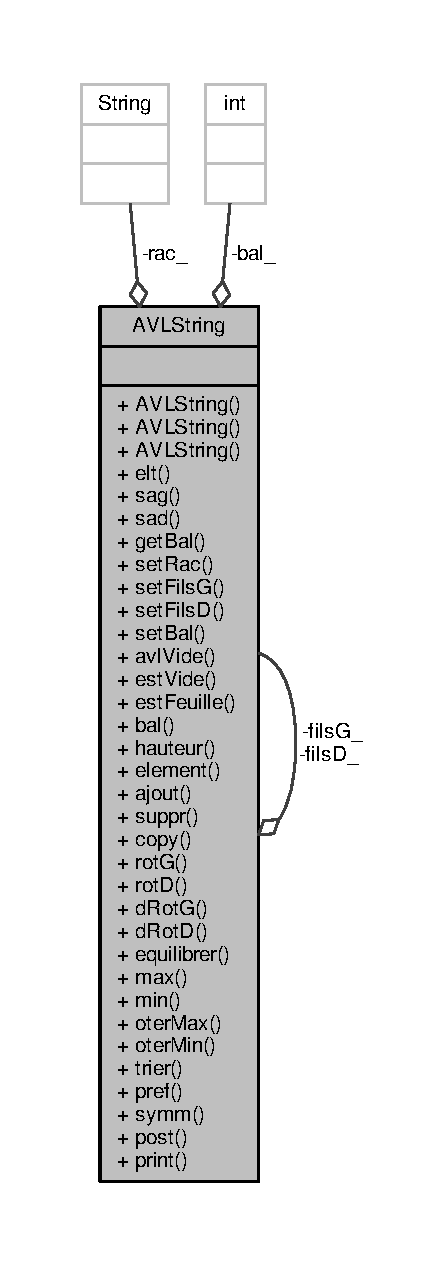
\includegraphics[height=550pt]{class_a_v_l_string__coll__graph}
\end{center}
\end{figure}
\subsection*{Public Member Functions}
\begin{DoxyCompactItemize}
\item 
\hyperlink{class_a_v_l_string_a7cae60ef637f6aad039371478fc5deed}{A\-V\-L\-String} ()
\item 
\hyperlink{class_a_v_l_string_a03a3566175c444bf44100d4b5ed8ae3e}{A\-V\-L\-String} (String rac)
\item 
\hyperlink{class_a_v_l_string_ad54ef293b3b066f1cfbcfd33b110a523}{A\-V\-L\-String} (String rac, \hyperlink{class_a_v_l_string}{A\-V\-L\-String} fils\-G, \hyperlink{class_a_v_l_string}{A\-V\-L\-String} fils\-D)
\item 
String \hyperlink{class_a_v_l_string_a04e9b58049f335c818886b69ae3ececc}{elt} ()
\item 
\hyperlink{class_a_v_l_string}{A\-V\-L\-String} \hyperlink{class_a_v_l_string_a0c2b74170cea4c3aae4859c9504f8440}{sag} ()
\item 
\hyperlink{class_a_v_l_string}{A\-V\-L\-String} \hyperlink{class_a_v_l_string_a5ed9a9d93f55b1691126934d33b7ff04}{sad} ()
\item 
int \hyperlink{class_a_v_l_string_a9b6514bbe1eeb60cd063038f633638a0}{get\-Bal} ()
\item 
void \hyperlink{class_a_v_l_string_aa1de0f428ebeb20058ac04f03f948220}{set\-Rac} (String rac)
\item 
void \hyperlink{class_a_v_l_string_ac4f52500381c77fb5ec4a1f30cc98f9c}{set\-Fils\-G} (\hyperlink{class_a_v_l_string}{A\-V\-L\-String} fils\-G)
\item 
void \hyperlink{class_a_v_l_string_afe2973bf4e0b311745d8a0e78ce37f87}{set\-Fils\-D} (\hyperlink{class_a_v_l_string}{A\-V\-L\-String} fils\-D)
\item 
void \hyperlink{class_a_v_l_string_af557c5f3b98c3df26a8866e89fd4e173}{set\-Bal} (int \hyperlink{class_a_v_l_string_ae45259bb6e0ecd30b7764c270f2421eb}{bal})
\item 
void \hyperlink{class_a_v_l_string_a822881c4be4ef7e6aada44f6b9b9487a}{avl\-Vide} ()
\item 
boolean \hyperlink{class_a_v_l_string_a82630baa2869275d044e3f25d40d52f7}{est\-Vide} ()
\item 
boolean \hyperlink{class_a_v_l_string_a5f0d9ef42d56854c6977b1e7e143197e}{est\-Feuille} ()
\item 
void \hyperlink{class_a_v_l_string_ae45259bb6e0ecd30b7764c270f2421eb}{bal} ()
\item 
int \hyperlink{class_a_v_l_string_aa452d84d47b7bf724362d5f856be3374}{hauteur} ()
\item 
boolean \hyperlink{class_a_v_l_string_abd6d41261357b2501fc805216f6eb456}{element} (String \hyperlink{class_a_v_l_string_a04e9b58049f335c818886b69ae3ececc}{elt})
\item 
int \hyperlink{class_a_v_l_string_a450d8ec3c60cf1a989f03112f4b9855d}{ajout} (String \hyperlink{class_a_v_l_string_a04e9b58049f335c818886b69ae3ececc}{elt})
\item 
int \hyperlink{class_a_v_l_string_a1f73174ef1b9a223d94e44719cc6736f}{suppr} (String \hyperlink{class_a_v_l_string_a04e9b58049f335c818886b69ae3ececc}{elt})
\item 
void \hyperlink{class_a_v_l_string_a738d9b71bb2ee680c2bebe547da683e7}{copy} (\hyperlink{class_a_v_l_string}{A\-V\-L\-String} av)
\item 
void \hyperlink{class_a_v_l_string_ad960ebcc3991cb679add72f3dda4caa0}{rot\-G} ()
\item 
void \hyperlink{class_a_v_l_string_a16e45537a756d78a0f54020e4ca3dd82}{rot\-D} ()
\item 
void \hyperlink{class_a_v_l_string_ae9bb040328e2fe9a02ae68178231cf41}{d\-Rot\-G} ()
\item 
void \hyperlink{class_a_v_l_string_a6234278e0d2587d5f899dc003c7d1de6}{d\-Rot\-D} ()
\item 
void \hyperlink{class_a_v_l_string_afd90cb3564177a7a37056164d039b0dd}{equilibrer} ()
\item 
String \hyperlink{class_a_v_l_string_aa1d9f436aa7766d5ec0498454f32dfe9}{max} ()
\item 
String \hyperlink{class_a_v_l_string_a9535c4d4517a1103149b348e1126765d}{min} ()
\item 
int \hyperlink{class_a_v_l_string_a5d47afdb15e0cf57f7e27c2f1e1a3c3d}{oter\-Max} ()
\item 
int \hyperlink{class_a_v_l_string_a4bb66e491eccfc0531239f57bf9b01f1}{oter\-Min} ()
\item 
Array\-List$<$ String $>$ \hyperlink{class_a_v_l_string_abe38e3948352fcffc2db0f066c3b97cf}{trier} (Array\-List$<$ String $>$ l)
\item 
Array\-List$<$ String $>$ \hyperlink{class_a_v_l_string_aa8e9250c0b5719b2f197e24c4be4b9e8}{pref} ()
\item 
Array\-List$<$ String $>$ \hyperlink{class_a_v_l_string_a0efe1dbea6307856f3b727df8663b66f}{symm} ()
\item 
Array\-List$<$ String $>$ \hyperlink{class_a_v_l_string_a11601b5dbb6e37215708938323364af7}{post} ()
\item 
String \hyperlink{class_a_v_l_string_adde3aa65616bf1c05ea2407ea8cb255f}{print} (int ch)
\end{DoxyCompactItemize}
\subsection*{Private Attributes}
\begin{DoxyCompactItemize}
\item 
String \hyperlink{class_a_v_l_string_adb167b91de2f634545354179d75c7a2a}{rac\-\_\-}
\item 
\hyperlink{class_a_v_l_string}{A\-V\-L\-String} \hyperlink{class_a_v_l_string_ad79e01875b56754629c8e0c928fcf530}{fils\-G\-\_\-}
\item 
\hyperlink{class_a_v_l_string}{A\-V\-L\-String} \hyperlink{class_a_v_l_string_a683f6fd78271d50b935b0255ffc7441a}{fils\-D\-\_\-}
\item 
int \hyperlink{class_a_v_l_string_a5a492e5ae84bdf492f68e1f41e918734}{bal\-\_\-}
\end{DoxyCompactItemize}


\subsection{Constructor \& Destructor Documentation}
\hypertarget{class_a_v_l_string_a7cae60ef637f6aad039371478fc5deed}{\index{A\-V\-L\-String@{A\-V\-L\-String}!A\-V\-L\-String@{A\-V\-L\-String}}
\index{A\-V\-L\-String@{A\-V\-L\-String}!AVLString@{A\-V\-L\-String}}
\subsubsection[{A\-V\-L\-String}]{\setlength{\rightskip}{0pt plus 5cm}A\-V\-L\-String.\-A\-V\-L\-String (
\begin{DoxyParamCaption}
{}
\end{DoxyParamCaption}
)}}\label{class_a_v_l_string_a7cae60ef637f6aad039371478fc5deed}
\mbox{[}\hyperlink{class_a_v_l_string}{A\-V\-L\-String} =$>$ Construit un A\-V\-L \char`\"{}vide\char`\"{}\mbox{]} \begin{DoxyReturn}{Returns}
\mbox{[}équivalent d'un A\-V\-L vide -\/$>$ racine et sous arbres non initialisés\mbox{]} 
\end{DoxyReturn}
\hypertarget{class_a_v_l_string_a03a3566175c444bf44100d4b5ed8ae3e}{\index{A\-V\-L\-String@{A\-V\-L\-String}!A\-V\-L\-String@{A\-V\-L\-String}}
\index{A\-V\-L\-String@{A\-V\-L\-String}!AVLString@{A\-V\-L\-String}}
\subsubsection[{A\-V\-L\-String}]{\setlength{\rightskip}{0pt plus 5cm}A\-V\-L\-String.\-A\-V\-L\-String (
\begin{DoxyParamCaption}
\item[{String}]{rac}
\end{DoxyParamCaption}
)}}\label{class_a_v_l_string_a03a3566175c444bf44100d4b5ed8ae3e}
\mbox{[}\hyperlink{class_a_v_l_string}{A\-V\-L\-String} =$>$ Construit un A\-V\-L \char`\"{}feuille\char`\"{}\mbox{]} 
\begin{DoxyParams}{Parameters}
{\em rac} & \mbox{[}valeur de la racine\mbox{]} \\
\hline
\end{DoxyParams}
\begin{DoxyReturn}{Returns}
\mbox{[}équivalent d'un A\-V\-L feuille -\/$>$ racine initialisée et sous-\/arbres vides\mbox{]} 
\end{DoxyReturn}
\hypertarget{class_a_v_l_string_ad54ef293b3b066f1cfbcfd33b110a523}{\index{A\-V\-L\-String@{A\-V\-L\-String}!A\-V\-L\-String@{A\-V\-L\-String}}
\index{A\-V\-L\-String@{A\-V\-L\-String}!AVLString@{A\-V\-L\-String}}
\subsubsection[{A\-V\-L\-String}]{\setlength{\rightskip}{0pt plus 5cm}A\-V\-L\-String.\-A\-V\-L\-String (
\begin{DoxyParamCaption}
\item[{String}]{rac, }
\item[{{\bf A\-V\-L\-String}}]{fils\-G, }
\item[{{\bf A\-V\-L\-String}}]{fils\-D}
\end{DoxyParamCaption}
)}}\label{class_a_v_l_string_ad54ef293b3b066f1cfbcfd33b110a523}
\mbox{[}\hyperlink{class_a_v_l_string}{A\-V\-L\-String} =$>$ Construit un A\-V\-L donc la forme dépendra des paramètres passés\mbox{]} 
\begin{DoxyParams}{Parameters}
{\em rac} & \mbox{[}valeur de la racine\mbox{]} \\
\hline
{\em fils\-G} & \mbox{[}A\-V\-L qui sera fils gauche\mbox{]} \\
\hline
{\em fils\-D} & \mbox{[}A\-V\-L qui sera fils droit\mbox{]} \\
\hline
\end{DoxyParams}
\begin{DoxyReturn}{Returns}
\mbox{[}A\-V\-L de forme quelconque, selon les paramètres passés\mbox{]} 
\end{DoxyReturn}


\subsection{Member Function Documentation}
\hypertarget{class_a_v_l_string_a450d8ec3c60cf1a989f03112f4b9855d}{\index{A\-V\-L\-String@{A\-V\-L\-String}!ajout@{ajout}}
\index{ajout@{ajout}!AVLString@{A\-V\-L\-String}}
\subsubsection[{ajout}]{\setlength{\rightskip}{0pt plus 5cm}int A\-V\-L\-String.\-ajout (
\begin{DoxyParamCaption}
\item[{String}]{elt}
\end{DoxyParamCaption}
)}}\label{class_a_v_l_string_a450d8ec3c60cf1a989f03112f4b9855d}
\mbox{[}ajout =$>$ Ajoute elt à l'A\-V\-L, et retourne la variation de hauteur\mbox{]} 
\begin{DoxyParams}{Parameters}
{\em elt} & \mbox{[}String\mbox{]} \\
\hline
\end{DoxyParams}
\begin{DoxyReturn}{Returns}
\mbox{[}entier\mbox{]} 
\end{DoxyReturn}
\hypertarget{class_a_v_l_string_a822881c4be4ef7e6aada44f6b9b9487a}{\index{A\-V\-L\-String@{A\-V\-L\-String}!avl\-Vide@{avl\-Vide}}
\index{avl\-Vide@{avl\-Vide}!AVLString@{A\-V\-L\-String}}
\subsubsection[{avl\-Vide}]{\setlength{\rightskip}{0pt plus 5cm}void A\-V\-L\-String.\-avl\-Vide (
\begin{DoxyParamCaption}
{}
\end{DoxyParamCaption}
)}}\label{class_a_v_l_string_a822881c4be4ef7e6aada44f6b9b9487a}
\mbox{[}avl\-Vide =$>$ Remplace l'A\-V\-L par un arbre vide\mbox{]} \hypertarget{class_a_v_l_string_ae45259bb6e0ecd30b7764c270f2421eb}{\index{A\-V\-L\-String@{A\-V\-L\-String}!bal@{bal}}
\index{bal@{bal}!AVLString@{A\-V\-L\-String}}
\subsubsection[{bal}]{\setlength{\rightskip}{0pt plus 5cm}void A\-V\-L\-String.\-bal (
\begin{DoxyParamCaption}
{}
\end{DoxyParamCaption}
)}}\label{class_a_v_l_string_ae45259bb6e0ecd30b7764c270f2421eb}
\mbox{[}bal =$>$ Recalcule récursivement la balance de l'A\-V\-L et celles de tous ses fils\mbox{]} \hypertarget{class_a_v_l_string_a738d9b71bb2ee680c2bebe547da683e7}{\index{A\-V\-L\-String@{A\-V\-L\-String}!copy@{copy}}
\index{copy@{copy}!AVLString@{A\-V\-L\-String}}
\subsubsection[{copy}]{\setlength{\rightskip}{0pt plus 5cm}void A\-V\-L\-String.\-copy (
\begin{DoxyParamCaption}
\item[{{\bf A\-V\-L\-String}}]{av}
\end{DoxyParamCaption}
)}}\label{class_a_v_l_string_a738d9b71bb2ee680c2bebe547da683e7}
\mbox{[}copy =$>$ Retourne une copie de l'A\-V\-L passé en paramètre\mbox{]} 
\begin{DoxyParams}{Parameters}
{\em av} & \mbox{[}A\-V\-L\mbox{]} \\
\hline
\end{DoxyParams}
\hypertarget{class_a_v_l_string_a6234278e0d2587d5f899dc003c7d1de6}{\index{A\-V\-L\-String@{A\-V\-L\-String}!d\-Rot\-D@{d\-Rot\-D}}
\index{d\-Rot\-D@{d\-Rot\-D}!AVLString@{A\-V\-L\-String}}
\subsubsection[{d\-Rot\-D}]{\setlength{\rightskip}{0pt plus 5cm}void A\-V\-L\-String.\-d\-Rot\-D (
\begin{DoxyParamCaption}
{}
\end{DoxyParamCaption}
)}}\label{class_a_v_l_string_a6234278e0d2587d5f899dc003c7d1de6}
\mbox{[}d\-Rot\-D =$>$ Effectue une double rotation droite sur l'A\-V\-L\mbox{]} \hypertarget{class_a_v_l_string_ae9bb040328e2fe9a02ae68178231cf41}{\index{A\-V\-L\-String@{A\-V\-L\-String}!d\-Rot\-G@{d\-Rot\-G}}
\index{d\-Rot\-G@{d\-Rot\-G}!AVLString@{A\-V\-L\-String}}
\subsubsection[{d\-Rot\-G}]{\setlength{\rightskip}{0pt plus 5cm}void A\-V\-L\-String.\-d\-Rot\-G (
\begin{DoxyParamCaption}
{}
\end{DoxyParamCaption}
)}}\label{class_a_v_l_string_ae9bb040328e2fe9a02ae68178231cf41}
\mbox{[}d\-Rot\-G =$>$ Effectue une double rotation gauche sur l'A\-V\-L\mbox{]} \hypertarget{class_a_v_l_string_abd6d41261357b2501fc805216f6eb456}{\index{A\-V\-L\-String@{A\-V\-L\-String}!element@{element}}
\index{element@{element}!AVLString@{A\-V\-L\-String}}
\subsubsection[{element}]{\setlength{\rightskip}{0pt plus 5cm}boolean A\-V\-L\-String.\-element (
\begin{DoxyParamCaption}
\item[{String}]{elt}
\end{DoxyParamCaption}
)}}\label{class_a_v_l_string_abd6d41261357b2501fc805216f6eb456}
\mbox{[}element =$>$ Renvoie vrai si elt est présent dans l'A\-V\-L, faux sinon\mbox{]} 
\begin{DoxyParams}{Parameters}
{\em elt} & \mbox{[}String\mbox{]} \\
\hline
\end{DoxyParams}
\begin{DoxyReturn}{Returns}
\mbox{[}booléen\mbox{]} 
\end{DoxyReturn}
\hypertarget{class_a_v_l_string_a04e9b58049f335c818886b69ae3ececc}{\index{A\-V\-L\-String@{A\-V\-L\-String}!elt@{elt}}
\index{elt@{elt}!AVLString@{A\-V\-L\-String}}
\subsubsection[{elt}]{\setlength{\rightskip}{0pt plus 5cm}String A\-V\-L\-String.\-elt (
\begin{DoxyParamCaption}
{}
\end{DoxyParamCaption}
)}}\label{class_a_v_l_string_a04e9b58049f335c818886b69ae3ececc}
\mbox{[}elt =$>$ Retourne la racine de l'A\-V\-L\mbox{]} \begin{DoxyReturn}{Returns}
\mbox{[}String (valeur de la racine)\mbox{]} 
\end{DoxyReturn}
\hypertarget{class_a_v_l_string_afd90cb3564177a7a37056164d039b0dd}{\index{A\-V\-L\-String@{A\-V\-L\-String}!equilibrer@{equilibrer}}
\index{equilibrer@{equilibrer}!AVLString@{A\-V\-L\-String}}
\subsubsection[{equilibrer}]{\setlength{\rightskip}{0pt plus 5cm}void A\-V\-L\-String.\-equilibrer (
\begin{DoxyParamCaption}
{}
\end{DoxyParamCaption}
)}}\label{class_a_v_l_string_afd90cb3564177a7a37056164d039b0dd}
\mbox{[}equilibrer =$>$ Méthode appellée pour équilibrer l'A\-V\-L après ajout ou suppression\mbox{]} \hypertarget{class_a_v_l_string_a5f0d9ef42d56854c6977b1e7e143197e}{\index{A\-V\-L\-String@{A\-V\-L\-String}!est\-Feuille@{est\-Feuille}}
\index{est\-Feuille@{est\-Feuille}!AVLString@{A\-V\-L\-String}}
\subsubsection[{est\-Feuille}]{\setlength{\rightskip}{0pt plus 5cm}boolean A\-V\-L\-String.\-est\-Feuille (
\begin{DoxyParamCaption}
{}
\end{DoxyParamCaption}
)}}\label{class_a_v_l_string_a5f0d9ef42d56854c6977b1e7e143197e}
\mbox{[}est\-Feuille =$>$ Renvoie vrai si l'A\-V\-L correspond à un A\-V\-L feuille, faux sinon\mbox{]} \begin{DoxyReturn}{Returns}
\mbox{[}booléen\mbox{]} 
\end{DoxyReturn}
\hypertarget{class_a_v_l_string_a82630baa2869275d044e3f25d40d52f7}{\index{A\-V\-L\-String@{A\-V\-L\-String}!est\-Vide@{est\-Vide}}
\index{est\-Vide@{est\-Vide}!AVLString@{A\-V\-L\-String}}
\subsubsection[{est\-Vide}]{\setlength{\rightskip}{0pt plus 5cm}boolean A\-V\-L\-String.\-est\-Vide (
\begin{DoxyParamCaption}
{}
\end{DoxyParamCaption}
)}}\label{class_a_v_l_string_a82630baa2869275d044e3f25d40d52f7}
\mbox{[}est\-Vide =$>$ Renvoie vrai si l'A\-V\-L est vide, faux sinon\mbox{]} \begin{DoxyReturn}{Returns}
\mbox{[}booléen\mbox{]} 
\end{DoxyReturn}
\hypertarget{class_a_v_l_string_a9b6514bbe1eeb60cd063038f633638a0}{\index{A\-V\-L\-String@{A\-V\-L\-String}!get\-Bal@{get\-Bal}}
\index{get\-Bal@{get\-Bal}!AVLString@{A\-V\-L\-String}}
\subsubsection[{get\-Bal}]{\setlength{\rightskip}{0pt plus 5cm}int A\-V\-L\-String.\-get\-Bal (
\begin{DoxyParamCaption}
{}
\end{DoxyParamCaption}
)}}\label{class_a_v_l_string_a9b6514bbe1eeb60cd063038f633638a0}
\mbox{[}get\-Bal =$>$ Retourne la balance de l'A\-V\-L\mbox{]} \begin{DoxyReturn}{Returns}
\mbox{[}entier (balance)\mbox{]} 
\end{DoxyReturn}
\hypertarget{class_a_v_l_string_aa452d84d47b7bf724362d5f856be3374}{\index{A\-V\-L\-String@{A\-V\-L\-String}!hauteur@{hauteur}}
\index{hauteur@{hauteur}!AVLString@{A\-V\-L\-String}}
\subsubsection[{hauteur}]{\setlength{\rightskip}{0pt plus 5cm}int A\-V\-L\-String.\-hauteur (
\begin{DoxyParamCaption}
{}
\end{DoxyParamCaption}
)}}\label{class_a_v_l_string_aa452d84d47b7bf724362d5f856be3374}
\mbox{[}hauteur =$>$ Renvoie la hauteur de l'A\-V\-L (la racine étant à la hauteur 0)\mbox{]} \begin{DoxyReturn}{Returns}
\mbox{[}entier\mbox{]} 
\end{DoxyReturn}
\hypertarget{class_a_v_l_string_aa1d9f436aa7766d5ec0498454f32dfe9}{\index{A\-V\-L\-String@{A\-V\-L\-String}!max@{max}}
\index{max@{max}!AVLString@{A\-V\-L\-String}}
\subsubsection[{max}]{\setlength{\rightskip}{0pt plus 5cm}String A\-V\-L\-String.\-max (
\begin{DoxyParamCaption}
{}
\end{DoxyParamCaption}
)}}\label{class_a_v_l_string_aa1d9f436aa7766d5ec0498454f32dfe9}
\mbox{[}max =$>$ Retourne le plus grand élément de l'A\-V\-L (-\/1 si l'A\-V\-L est vide)\mbox{]} \begin{DoxyReturn}{Returns}
\mbox{[}entier\mbox{]} 
\end{DoxyReturn}
\hypertarget{class_a_v_l_string_a9535c4d4517a1103149b348e1126765d}{\index{A\-V\-L\-String@{A\-V\-L\-String}!min@{min}}
\index{min@{min}!AVLString@{A\-V\-L\-String}}
\subsubsection[{min}]{\setlength{\rightskip}{0pt plus 5cm}String A\-V\-L\-String.\-min (
\begin{DoxyParamCaption}
{}
\end{DoxyParamCaption}
)}}\label{class_a_v_l_string_a9535c4d4517a1103149b348e1126765d}
\mbox{[}min =$>$ Retourne le plus petit élément de l'A\-V\-L (\char`\"{}!\char`\"{} si l'A\-V\-L est vide)\mbox{]}\mbox{]} \begin{DoxyReturn}{Returns}
\mbox{[}entier\mbox{]} 
\end{DoxyReturn}
\hypertarget{class_a_v_l_string_a5d47afdb15e0cf57f7e27c2f1e1a3c3d}{\index{A\-V\-L\-String@{A\-V\-L\-String}!oter\-Max@{oter\-Max}}
\index{oter\-Max@{oter\-Max}!AVLString@{A\-V\-L\-String}}
\subsubsection[{oter\-Max}]{\setlength{\rightskip}{0pt plus 5cm}int A\-V\-L\-String.\-oter\-Max (
\begin{DoxyParamCaption}
{}
\end{DoxyParamCaption}
)}}\label{class_a_v_l_string_a5d47afdb15e0cf57f7e27c2f1e1a3c3d}
\mbox{[}oter\-Max =$>$ Retire le noeud contenant le plus grand élément de l'A\-V\-L (si celui-\/ci n'est pas vide)\mbox{]} \begin{DoxyReturn}{Returns}
\mbox{[}entier (correspondant à la variation de hauteur)\mbox{]} 
\end{DoxyReturn}
\hypertarget{class_a_v_l_string_a4bb66e491eccfc0531239f57bf9b01f1}{\index{A\-V\-L\-String@{A\-V\-L\-String}!oter\-Min@{oter\-Min}}
\index{oter\-Min@{oter\-Min}!AVLString@{A\-V\-L\-String}}
\subsubsection[{oter\-Min}]{\setlength{\rightskip}{0pt plus 5cm}int A\-V\-L\-String.\-oter\-Min (
\begin{DoxyParamCaption}
{}
\end{DoxyParamCaption}
)}}\label{class_a_v_l_string_a4bb66e491eccfc0531239f57bf9b01f1}
\mbox{[}oter\-Min =$>$ Retire le noeud contenant le plus petit élément de l'A\-V\-L (si celui-\/ci n'est pas vide)\mbox{]} \begin{DoxyReturn}{Returns}
\mbox{[}entier (correspondant à la variation de hauteur)\mbox{]} 
\end{DoxyReturn}
\hypertarget{class_a_v_l_string_a11601b5dbb6e37215708938323364af7}{\index{A\-V\-L\-String@{A\-V\-L\-String}!post@{post}}
\index{post@{post}!AVLString@{A\-V\-L\-String}}
\subsubsection[{post}]{\setlength{\rightskip}{0pt plus 5cm}Array\-List$<$String$>$ A\-V\-L\-String.\-post (
\begin{DoxyParamCaption}
{}
\end{DoxyParamCaption}
)}}\label{class_a_v_l_string_a11601b5dbb6e37215708938323364af7}
\mbox{[}post =$>$ Retourne le parcours postfixe de l'A\-V\-L\mbox{]} \begin{DoxyReturn}{Returns}
\mbox{[}Array\-List$<$\-String$>$\mbox{]} 
\end{DoxyReturn}
\hypertarget{class_a_v_l_string_aa8e9250c0b5719b2f197e24c4be4b9e8}{\index{A\-V\-L\-String@{A\-V\-L\-String}!pref@{pref}}
\index{pref@{pref}!AVLString@{A\-V\-L\-String}}
\subsubsection[{pref}]{\setlength{\rightskip}{0pt plus 5cm}Array\-List$<$String$>$ A\-V\-L\-String.\-pref (
\begin{DoxyParamCaption}
{}
\end{DoxyParamCaption}
)}}\label{class_a_v_l_string_aa8e9250c0b5719b2f197e24c4be4b9e8}
\mbox{[}pref =$>$ Retourne le parcours préfixe de l'A\-V\-L\mbox{]} \begin{DoxyReturn}{Returns}
\mbox{[}Array\-List$<$\-String$>$\mbox{]} 
\end{DoxyReturn}
\hypertarget{class_a_v_l_string_adde3aa65616bf1c05ea2407ea8cb255f}{\index{A\-V\-L\-String@{A\-V\-L\-String}!print@{print}}
\index{print@{print}!AVLString@{A\-V\-L\-String}}
\subsubsection[{print}]{\setlength{\rightskip}{0pt plus 5cm}String A\-V\-L\-String.\-print (
\begin{DoxyParamCaption}
\item[{int}]{ch}
\end{DoxyParamCaption}
)}}\label{class_a_v_l_string_adde3aa65616bf1c05ea2407ea8cb255f}
\mbox{[}print =$>$ Renvoie une chaîne représentant l'A\-V\-L en liste par son parcours préfixe, symétrique ou postfixe selon la valeur de l'entier passé en paramètre\mbox{]} 
\begin{DoxyParams}{Parameters}
{\em ch} & \mbox{[}entier, définissant le parcours devant être utilisé pour représenter l'A\-V\-L\mbox{]} si ch == 1 \-: parcours préfixe si ch == 2 \-: parcours symétrique si ch == 3 \-: parcours postfixe \\
\hline
\end{DoxyParams}
\begin{DoxyReturn}{Returns}
\mbox{[}chaîne de caractères\mbox{]} 
\end{DoxyReturn}
\hypertarget{class_a_v_l_string_a16e45537a756d78a0f54020e4ca3dd82}{\index{A\-V\-L\-String@{A\-V\-L\-String}!rot\-D@{rot\-D}}
\index{rot\-D@{rot\-D}!AVLString@{A\-V\-L\-String}}
\subsubsection[{rot\-D}]{\setlength{\rightskip}{0pt plus 5cm}void A\-V\-L\-String.\-rot\-D (
\begin{DoxyParamCaption}
{}
\end{DoxyParamCaption}
)}}\label{class_a_v_l_string_a16e45537a756d78a0f54020e4ca3dd82}
\mbox{[}rot\-D =$>$ Effectue une rotation droite (simple) sur l'A\-V\-L\mbox{]} \hypertarget{class_a_v_l_string_ad960ebcc3991cb679add72f3dda4caa0}{\index{A\-V\-L\-String@{A\-V\-L\-String}!rot\-G@{rot\-G}}
\index{rot\-G@{rot\-G}!AVLString@{A\-V\-L\-String}}
\subsubsection[{rot\-G}]{\setlength{\rightskip}{0pt plus 5cm}void A\-V\-L\-String.\-rot\-G (
\begin{DoxyParamCaption}
{}
\end{DoxyParamCaption}
)}}\label{class_a_v_l_string_ad960ebcc3991cb679add72f3dda4caa0}
\mbox{[}rot\-G =$>$ Effectue une rotation gauche (simple) sur l'A\-V\-L\mbox{]} \hypertarget{class_a_v_l_string_a5ed9a9d93f55b1691126934d33b7ff04}{\index{A\-V\-L\-String@{A\-V\-L\-String}!sad@{sad}}
\index{sad@{sad}!AVLString@{A\-V\-L\-String}}
\subsubsection[{sad}]{\setlength{\rightskip}{0pt plus 5cm}{\bf A\-V\-L\-String} A\-V\-L\-String.\-sad (
\begin{DoxyParamCaption}
{}
\end{DoxyParamCaption}
)}}\label{class_a_v_l_string_a5ed9a9d93f55b1691126934d33b7ff04}
\mbox{[}sad =$>$ Retourne le sous-\/arbre droit de l'A\-V\-L\mbox{]} \begin{DoxyReturn}{Returns}
\mbox{[}A\-V\-L (sous-\/arbre droit)\mbox{]} 
\end{DoxyReturn}
\hypertarget{class_a_v_l_string_a0c2b74170cea4c3aae4859c9504f8440}{\index{A\-V\-L\-String@{A\-V\-L\-String}!sag@{sag}}
\index{sag@{sag}!AVLString@{A\-V\-L\-String}}
\subsubsection[{sag}]{\setlength{\rightskip}{0pt plus 5cm}{\bf A\-V\-L\-String} A\-V\-L\-String.\-sag (
\begin{DoxyParamCaption}
{}
\end{DoxyParamCaption}
)}}\label{class_a_v_l_string_a0c2b74170cea4c3aae4859c9504f8440}
\mbox{[}sag =$>$ Retourne le sous-\/arbre gauche de l'A\-V\-L\mbox{]} \begin{DoxyReturn}{Returns}
\mbox{[}A\-V\-L (sous-\/arbre gauche)\mbox{]} 
\end{DoxyReturn}
\hypertarget{class_a_v_l_string_af557c5f3b98c3df26a8866e89fd4e173}{\index{A\-V\-L\-String@{A\-V\-L\-String}!set\-Bal@{set\-Bal}}
\index{set\-Bal@{set\-Bal}!AVLString@{A\-V\-L\-String}}
\subsubsection[{set\-Bal}]{\setlength{\rightskip}{0pt plus 5cm}void A\-V\-L\-String.\-set\-Bal (
\begin{DoxyParamCaption}
\item[{int}]{bal}
\end{DoxyParamCaption}
)}}\label{class_a_v_l_string_af557c5f3b98c3df26a8866e89fd4e173}
\mbox{[}set\-Bal =$>$ Remplace la balance\mbox{]} 
\begin{DoxyParams}{Parameters}
{\em bal} & \mbox{[}entier\mbox{]} \\
\hline
\end{DoxyParams}
\hypertarget{class_a_v_l_string_afe2973bf4e0b311745d8a0e78ce37f87}{\index{A\-V\-L\-String@{A\-V\-L\-String}!set\-Fils\-D@{set\-Fils\-D}}
\index{set\-Fils\-D@{set\-Fils\-D}!AVLString@{A\-V\-L\-String}}
\subsubsection[{set\-Fils\-D}]{\setlength{\rightskip}{0pt plus 5cm}void A\-V\-L\-String.\-set\-Fils\-D (
\begin{DoxyParamCaption}
\item[{{\bf A\-V\-L\-String}}]{fils\-D}
\end{DoxyParamCaption}
)}}\label{class_a_v_l_string_afe2973bf4e0b311745d8a0e78ce37f87}
\mbox{[}set\-Fils\-D =$>$ Remplace le fils droit\mbox{]} 
\begin{DoxyParams}{Parameters}
{\em fils\-D} & \mbox{[}A\-V\-L\mbox{]} \\
\hline
\end{DoxyParams}
\hypertarget{class_a_v_l_string_ac4f52500381c77fb5ec4a1f30cc98f9c}{\index{A\-V\-L\-String@{A\-V\-L\-String}!set\-Fils\-G@{set\-Fils\-G}}
\index{set\-Fils\-G@{set\-Fils\-G}!AVLString@{A\-V\-L\-String}}
\subsubsection[{set\-Fils\-G}]{\setlength{\rightskip}{0pt plus 5cm}void A\-V\-L\-String.\-set\-Fils\-G (
\begin{DoxyParamCaption}
\item[{{\bf A\-V\-L\-String}}]{fils\-G}
\end{DoxyParamCaption}
)}}\label{class_a_v_l_string_ac4f52500381c77fb5ec4a1f30cc98f9c}
\mbox{[}set\-Fils\-G =$>$ Remplace le fils gauche\mbox{]} 
\begin{DoxyParams}{Parameters}
{\em fils\-G} & \mbox{[}A\-V\-L\mbox{]} \\
\hline
\end{DoxyParams}
\hypertarget{class_a_v_l_string_aa1de0f428ebeb20058ac04f03f948220}{\index{A\-V\-L\-String@{A\-V\-L\-String}!set\-Rac@{set\-Rac}}
\index{set\-Rac@{set\-Rac}!AVLString@{A\-V\-L\-String}}
\subsubsection[{set\-Rac}]{\setlength{\rightskip}{0pt plus 5cm}void A\-V\-L\-String.\-set\-Rac (
\begin{DoxyParamCaption}
\item[{String}]{rac}
\end{DoxyParamCaption}
)}}\label{class_a_v_l_string_aa1de0f428ebeb20058ac04f03f948220}
\mbox{[}set\-Rac =$>$ Remplace la valeur de la racine\mbox{]} 
\begin{DoxyParams}{Parameters}
{\em rac} & \mbox{[}String\mbox{]} \\
\hline
\end{DoxyParams}
\hypertarget{class_a_v_l_string_a1f73174ef1b9a223d94e44719cc6736f}{\index{A\-V\-L\-String@{A\-V\-L\-String}!suppr@{suppr}}
\index{suppr@{suppr}!AVLString@{A\-V\-L\-String}}
\subsubsection[{suppr}]{\setlength{\rightskip}{0pt plus 5cm}int A\-V\-L\-String.\-suppr (
\begin{DoxyParamCaption}
\item[{String}]{elt}
\end{DoxyParamCaption}
)}}\label{class_a_v_l_string_a1f73174ef1b9a223d94e44719cc6736f}
\mbox{[}suppr =$>$ Retire le noeud ayant elt pour élément de l'A\-V\-L (s'il existe)\mbox{]} 
\begin{DoxyParams}{Parameters}
{\em elt} & \mbox{[}String\mbox{]} \\
\hline
\end{DoxyParams}
\hypertarget{class_a_v_l_string_a0efe1dbea6307856f3b727df8663b66f}{\index{A\-V\-L\-String@{A\-V\-L\-String}!symm@{symm}}
\index{symm@{symm}!AVLString@{A\-V\-L\-String}}
\subsubsection[{symm}]{\setlength{\rightskip}{0pt plus 5cm}Array\-List$<$String$>$ A\-V\-L\-String.\-symm (
\begin{DoxyParamCaption}
{}
\end{DoxyParamCaption}
)}}\label{class_a_v_l_string_a0efe1dbea6307856f3b727df8663b66f}
\mbox{[}symm =$>$ Retourne le parcours symétrique de l'A\-V\-L\mbox{]} \begin{DoxyReturn}{Returns}
\mbox{[}Array\-List$<$\-String$>$\mbox{]} 
\end{DoxyReturn}
\hypertarget{class_a_v_l_string_abe38e3948352fcffc2db0f066c3b97cf}{\index{A\-V\-L\-String@{A\-V\-L\-String}!trier@{trier}}
\index{trier@{trier}!AVLString@{A\-V\-L\-String}}
\subsubsection[{trier}]{\setlength{\rightskip}{0pt plus 5cm}Array\-List$<$String$>$ A\-V\-L\-String.\-trier (
\begin{DoxyParamCaption}
\item[{Array\-List$<$ String $>$}]{l}
\end{DoxyParamCaption}
)}}\label{class_a_v_l_string_abe38e3948352fcffc2db0f066c3b97cf}
\mbox{[}trier =$>$ Trie une liste de String en utilisant un A\-V\-L (ordre lexicographique)\mbox{]} N\-B\-: La méthode n'utilise pas l'A\-V\-L auquel la méthode est appliquée au cas ou celui-\/ci ne serait pas vide, ce qui fausserait le résultat 
\begin{DoxyParams}{Parameters}
{\em l} & \mbox{[}Array\-List$<$\-String$>$ liste de Strings dont l'ordre est quelconque\mbox{]} \\
\hline
\end{DoxyParams}
\begin{DoxyReturn}{Returns}
\mbox{[}Array\-List$<$\-String$>$ liste de Strings triées par ordre croissant\mbox{]} 
\end{DoxyReturn}


\subsection{Member Data Documentation}
\hypertarget{class_a_v_l_string_a5a492e5ae84bdf492f68e1f41e918734}{\index{A\-V\-L\-String@{A\-V\-L\-String}!bal\-\_\-@{bal\-\_\-}}
\index{bal\-\_\-@{bal\-\_\-}!AVLString@{A\-V\-L\-String}}
\subsubsection[{bal\-\_\-}]{\setlength{\rightskip}{0pt plus 5cm}int A\-V\-L\-String.\-bal\-\_\-\hspace{0.3cm}{\ttfamily [private]}}}\label{class_a_v_l_string_a5a492e5ae84bdf492f68e1f41e918734}
balance -\/$>$ entier \hypertarget{class_a_v_l_string_a683f6fd78271d50b935b0255ffc7441a}{\index{A\-V\-L\-String@{A\-V\-L\-String}!fils\-D\-\_\-@{fils\-D\-\_\-}}
\index{fils\-D\-\_\-@{fils\-D\-\_\-}!AVLString@{A\-V\-L\-String}}
\subsubsection[{fils\-D\-\_\-}]{\setlength{\rightskip}{0pt plus 5cm}{\bf A\-V\-L\-String} A\-V\-L\-String.\-fils\-D\-\_\-\hspace{0.3cm}{\ttfamily [private]}}}\label{class_a_v_l_string_a683f6fd78271d50b935b0255ffc7441a}
fils droit -\/$>$ lui-\/même A\-V\-L \hypertarget{class_a_v_l_string_ad79e01875b56754629c8e0c928fcf530}{\index{A\-V\-L\-String@{A\-V\-L\-String}!fils\-G\-\_\-@{fils\-G\-\_\-}}
\index{fils\-G\-\_\-@{fils\-G\-\_\-}!AVLString@{A\-V\-L\-String}}
\subsubsection[{fils\-G\-\_\-}]{\setlength{\rightskip}{0pt plus 5cm}{\bf A\-V\-L\-String} A\-V\-L\-String.\-fils\-G\-\_\-\hspace{0.3cm}{\ttfamily [private]}}}\label{class_a_v_l_string_ad79e01875b56754629c8e0c928fcf530}
fils gauche -\/$>$ lui-\/même A\-V\-L \hypertarget{class_a_v_l_string_adb167b91de2f634545354179d75c7a2a}{\index{A\-V\-L\-String@{A\-V\-L\-String}!rac\-\_\-@{rac\-\_\-}}
\index{rac\-\_\-@{rac\-\_\-}!AVLString@{A\-V\-L\-String}}
\subsubsection[{rac\-\_\-}]{\setlength{\rightskip}{0pt plus 5cm}String A\-V\-L\-String.\-rac\-\_\-\hspace{0.3cm}{\ttfamily [private]}}}\label{class_a_v_l_string_adb167b91de2f634545354179d75c7a2a}
racine String 

The documentation for this class was generated from the following file\-:\begin{DoxyCompactItemize}
\item 
\hyperlink{_a_v_l_string_8java}{A\-V\-L\-String.\-java}\end{DoxyCompactItemize}

\hypertarget{class_test_a_v_l_string}{\section{Test\-A\-V\-L\-String Class Reference}
\label{class_test_a_v_l_string}\index{Test\-A\-V\-L\-String@{Test\-A\-V\-L\-String}}
}


Collaboration diagram for Test\-A\-V\-L\-String\-:\nopagebreak
\begin{figure}[H]
\begin{center}
\leavevmode
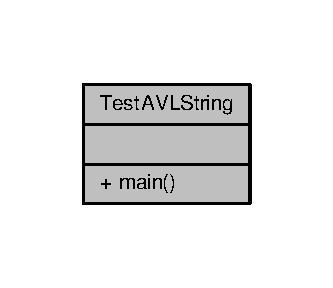
\includegraphics[width=160pt]{class_test_a_v_l_string__coll__graph}
\end{center}
\end{figure}
\subsection*{Static Public Member Functions}
\begin{DoxyCompactItemize}
\item 
static void \hyperlink{class_test_a_v_l_string_aeb4da230c4e739cd26106f6bafcdbc59}{main} (String args\mbox{[}$\,$\mbox{]})
\end{DoxyCompactItemize}


\subsection{Member Function Documentation}
\hypertarget{class_test_a_v_l_string_aeb4da230c4e739cd26106f6bafcdbc59}{\index{Test\-A\-V\-L\-String@{Test\-A\-V\-L\-String}!main@{main}}
\index{main@{main}!TestAVLString@{Test\-A\-V\-L\-String}}
\subsubsection[{main}]{\setlength{\rightskip}{0pt plus 5cm}static void Test\-A\-V\-L\-String.\-main (
\begin{DoxyParamCaption}
\item[{String}]{args\mbox{[}$\,$\mbox{]}}
\end{DoxyParamCaption}
)\hspace{0.3cm}{\ttfamily [static]}}}\label{class_test_a_v_l_string_aeb4da230c4e739cd26106f6bafcdbc59}


The documentation for this class was generated from the following file\-:\begin{DoxyCompactItemize}
\item 
\hyperlink{_test_a_v_l_string_8java}{Test\-A\-V\-L\-String.\-java}\end{DoxyCompactItemize}

\chapter{File Documentation}
\hypertarget{_a_v_l_string_8java}{\section{A\-V\-L\-String.\-java File Reference}
\label{_a_v_l_string_8java}\index{A\-V\-L\-String.\-java@{A\-V\-L\-String.\-java}}
}
\subsection*{Classes}
\begin{DoxyCompactItemize}
\item 
class \hyperlink{class_a_v_l_string}{A\-V\-L\-String}
\end{DoxyCompactItemize}

\hypertarget{_test_a_v_l_string_8java}{\section{Test\-A\-V\-L\-String.\-java File Reference}
\label{_test_a_v_l_string_8java}\index{Test\-A\-V\-L\-String.\-java@{Test\-A\-V\-L\-String.\-java}}
}
\subsection*{Classes}
\begin{DoxyCompactItemize}
\item 
class \hyperlink{class_test_a_v_l_string}{Test\-A\-V\-L\-String}
\end{DoxyCompactItemize}

%--- End generated contents ---

% Index
\newpage
\phantomsection
\addcontentsline{toc}{chapter}{Index}
\printindex

\end{document}
